\documentclass[a4paper, 11pt]{article}

%%%%%%%%%%%%
% Packages %
%%%%%%%%%%%%
\usepackage[utf8]{inputenc}
\usepackage[english]{babel}
\usepackage[margin=2.5cm]{geometry} % Standard margins
\usepackage{amsmath}  % For math
\usepackage{amssymb}  % For symbols
\usepackage{graphicx} % For images
\usepackage{booktabs} % For professional tables
\usepackage{subcaption} % For side-by-side images (subfigures)
\usepackage{float}    % For precise image placement [H]
\usepackage{hyperref} % For clickable links
\usepackage{parskip}  % Adds space between paragraphs instead of indentation
\usepackage{tikz}
\usepackage{tcolorbox}
\usepackage{xcolor}
% Packages



\usepackage{listings}
\usepackage{pgfplots}

\usetikzlibrary{shapes.geometric, arrows.meta, positioning, calc, fit, backgrounds, decorations.pathreplacing}
\pgfplotsset{compat=1.18}

% Custom colors
\definecolor{cudagreen}{RGB}{118,185,0}
\definecolor{cudablue}{RGB}{0,114,188}
\definecolor{cudaorange}{RGB}{255,127,0}
\definecolor{warpdiv}{RGB}{220,50,50}
\definecolor{sharedmem}{RGB}{255,215,0}
\definecolor{globalmem}{RGB}{100,149,237}
\definecolor{codebg}{RGB}{248,248,248}
\definecolor{codegreen}{rgb}{0,0.6,0}
\definecolor{codegray}{rgb}{0.5,0.5,0.5}
\definecolor{codepurple}{rgb}{0.58,0,0.82}

% Setup hyperlinks to look professional (blue, no boxes)
\hypersetup{
    colorlinks=true,
    linkcolor=blue,
    filecolor=magenta,      
    urlcolor=cyan,
    citecolor=blue
}

%%%%%%%%%%
% Macros %
%%%%%%%%%%
\newcommand{\ttbf}[1]{\texttt{\textbf{#1}}}

%%%%%%%%%%%%%%%%
% Title Details %
%%%%%%%%%%%%%%%%
\title{
    \textbf{Machine Learning Systems and Hardware (COMP70114)}\\
    \large Coursework: CUDA Kernel Development Report
}
\author{
    \textbf{Author}\\
    Anas Khan\\
    % \\
    % \textit{Imperial College London} \\
    % \textit{Department of Computer Science}
}
\date{\today}

%%%%%%%%%%%%
% Document %
%%%%%%%%%%%%

\begin{document}

\maketitle

% Optional: Abstract or Table of Contents could go here
% \tableofcontents
% \newpage
\vspace{-3em}
\section{Introduction: Part 1}
\vspace{-0.5em}
This report details our approach towards implementing Batch Normalisation Inference for tensors in NCHW (Batch, Channel, Height, Weight) memory layout using a CUDA kernel. 

\subsection{Correctness and Performance Metrics}

We were able to achieve the \textbf{Time Cost} of \textbf{0.983\,ms} through this implementation which passed all test cases with efficiently across all the benchmarks (see Figure~\ref{fig:batchnormresult}).  
\vspace{-4em}
\begin{figure}[H]
    \centering
    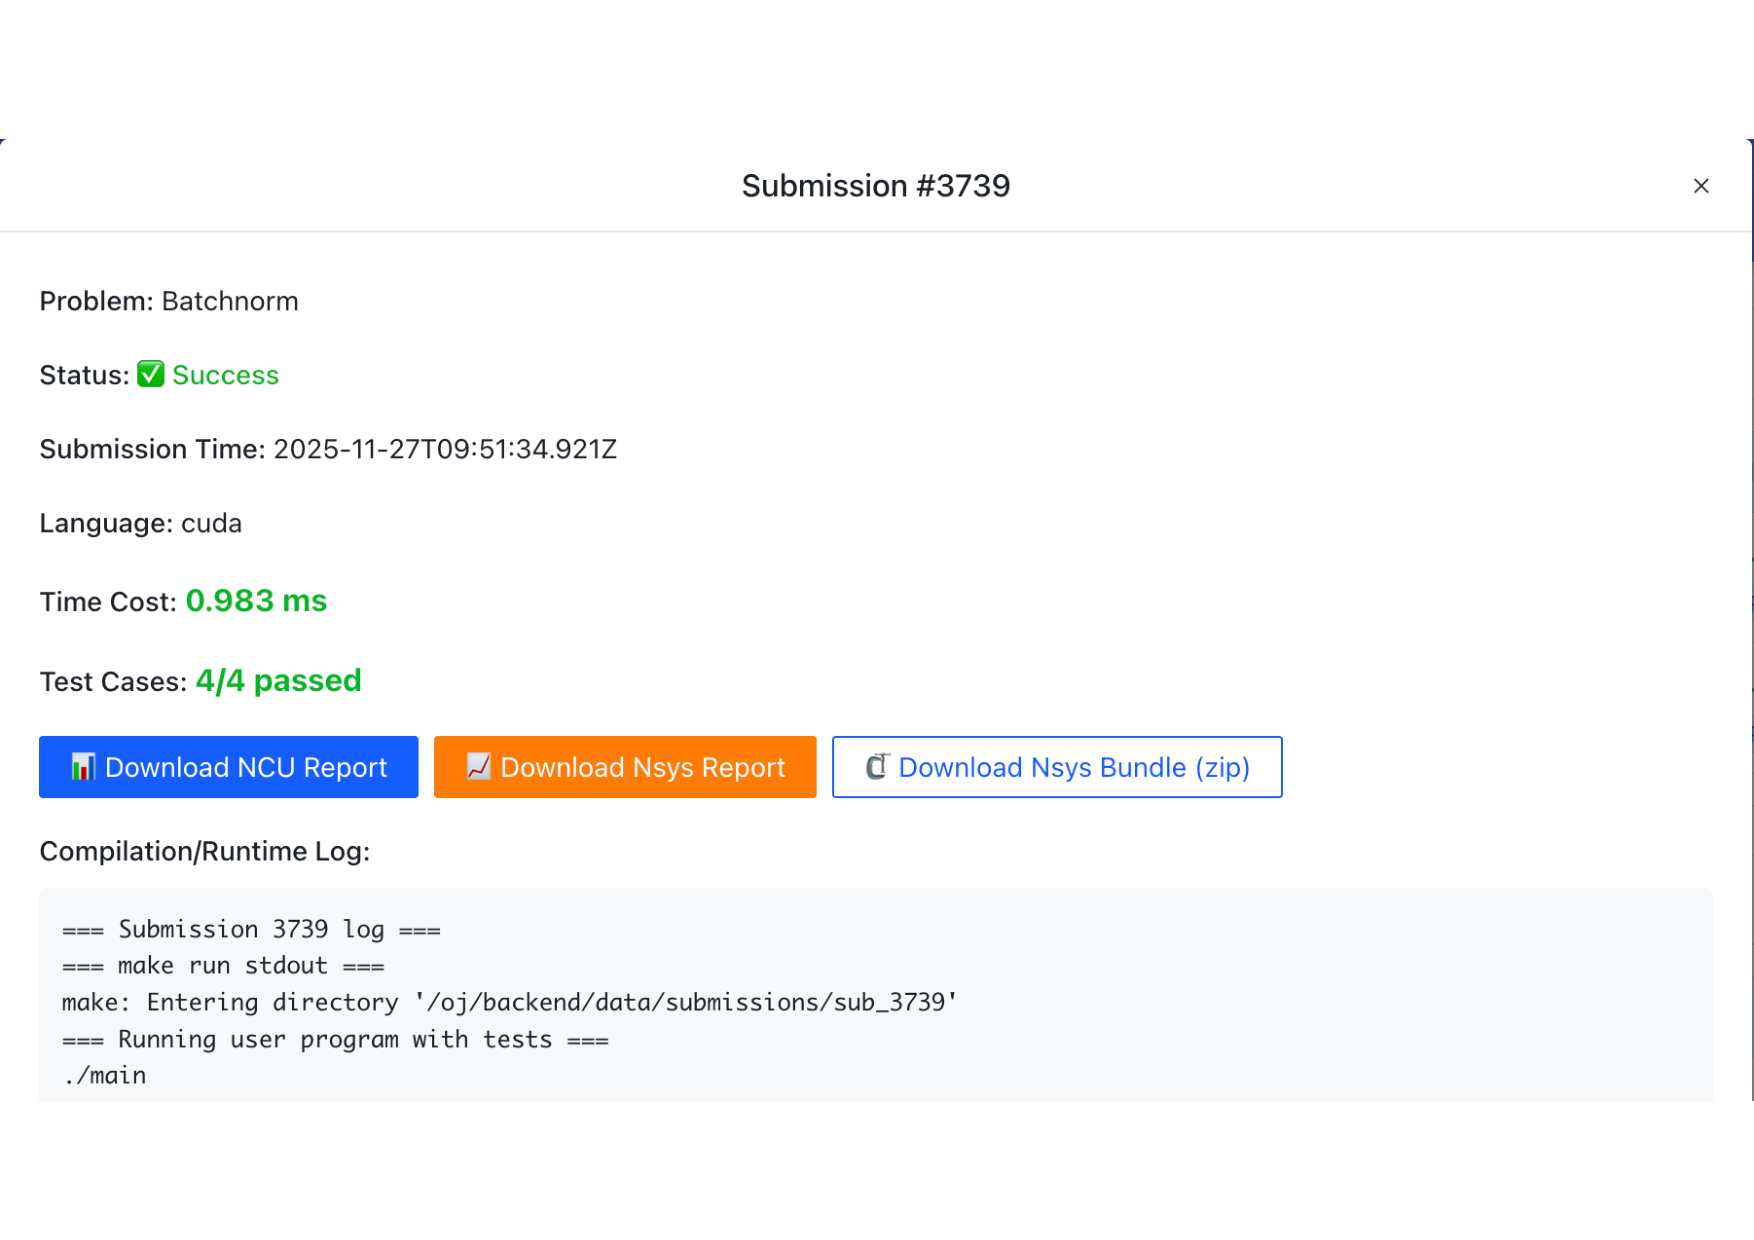
\includegraphics[width=\linewidth]{resources/Batchnorm-CUDA-Submission-AnasKhan.pdf}
    \caption{The evaluation of the problem one achieved a time cost of 0.983ms}
    \label{fig:batchnormresult}
\end{figure}
\vspace{-2em}
\subsection{Brief Implementation Explanation}

\begin{itemize}


    \item \textbf{Architectural Strategy (One-Block-Per-Channel):} The grid dimension was $(C, 1, 1)$. This mapped one CUDA Thread Block distinctively to one Feature Channel. This approach allowed a block to stay alive to process the entire spatial ($H \times W$) and batch ($N$) domain for that specific channel.
    
    \item \textbf{Vectorised Global Memory Access (Memory Coalescing):} The use of the input pointer to \texttt{float4*} allowed each thread to load 4 conseuctive floaring point (16 bytes) in a single function.

    \item \textbf{Register-Level Accumulation (Loop Unrolling):} During the accumulation phase, the sums and squared sums are stored in local registers rather than wrting into shared memory. This reduces shared memory bank conflicts.
\end{itemize}

\section{Introduction: Part 2}
\vspace{-0.5em}
In the second part the kernel, implements a direct standard convolution algorithm optimized for \textit{Depthwise} layers. In a Depthwise 2D Convolution, the channel interaction is removed; each input channel is convolved with its own unique 2D filter to produce one output channel.
\vspace{-6.5em}
\begin{figure}[H]
    \centering
    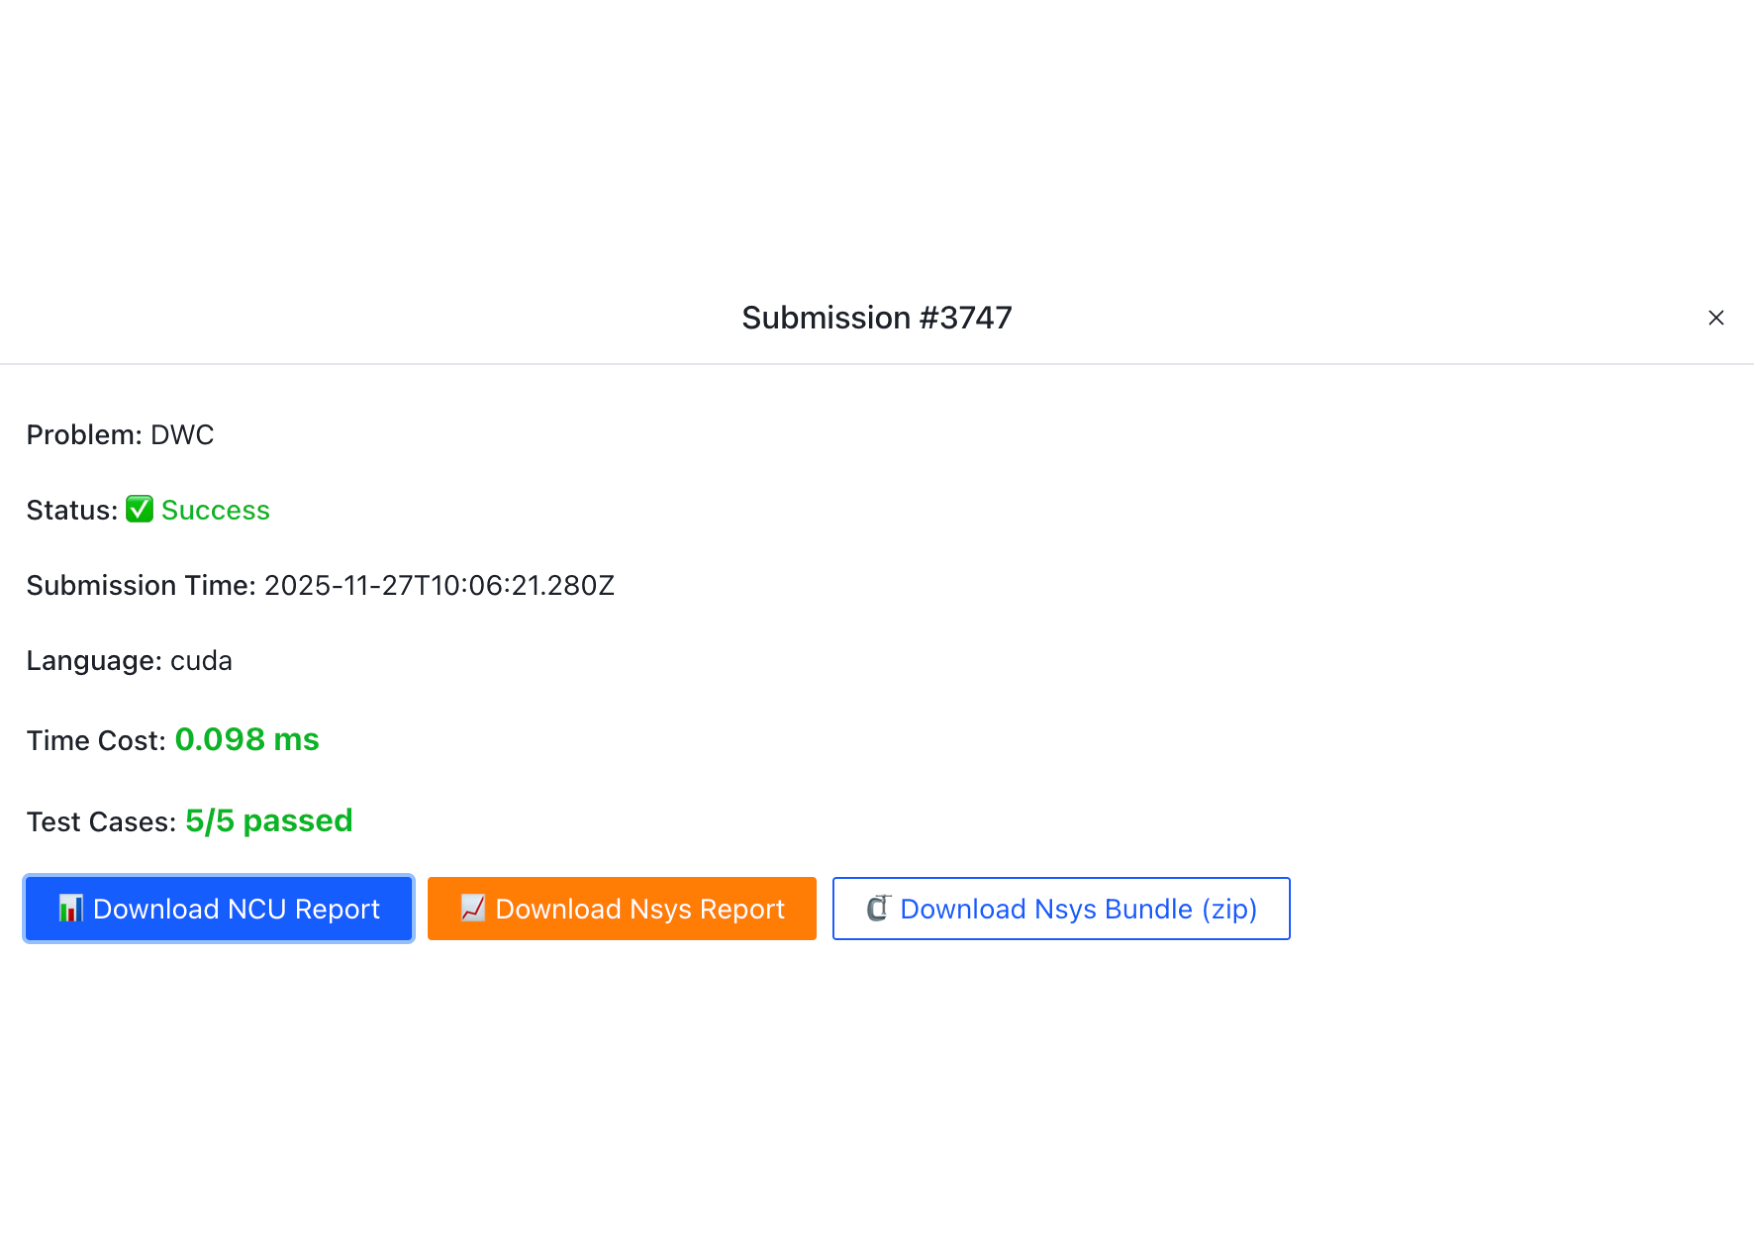
\includegraphics[width=\linewidth]{resources/AnasKhan_DWC_Submission_Eval.pdf}
    \caption{The evaluation of the problem two achieved a time cost of 0.098ms}
    \label{fig:dwcevalresult}
\end{figure}

\vspace{-2em}
\subsection{Correctness and Performance Metrics}

The best submission passed all the test cases efficiently and achieved a promising execution time of \textbf{0.098\,ms} (see Figure~\ref{fig:dwcevalresult}).


\subsection{Brief Implementation Explanation}

\begin{itemize}
    \item The kernel employs a \textbf{One-Thread-Per-Output-Pixel} strategy. This is a common baseline approach where parallelism is achieved by assigning independent threads to calculate every single pixel in the output tensor $Y$.

This mapping ensures that every output pixel is computed by exactly one thread, avoiding race conditions (no atomics needed).

\item Global Memory Access Pattern:
The spatial indexing strategy ($x$ dimension maps to $OW$) promotes memory coalescing. 

When loading $x$, threads access $x[\dots + (ow \cdot stride + kw)]$. If $stride=1$, these are perfectly contiguous addresses.

\end{itemize}

\vspace{1em}

\end{document}
